\documentclass{beamer}
\usetheme{Madrid}
\usepackage[italian]{babel}

\title[Trading AI]{Progettazione e sviluppo di test suite automatica e modulo raccolta dati per intelligenze artificiali che si occupano di creare strategie di investimento}
\author{Garion Musetta}
\centering
\date{Aprile 2020}
\begin{document}
\maketitle

\begin{frame}{Contesto}
\begin{itemize}
\item Nexid Edge blockchain e AI sviluppa strumenti intelligenti per l’analisi del mercato delle criptovalute e
la creazione di strategie di investimento.\\ Inoltre realizza Smart Contract sulla Blockchain Ethereum per la certificazione di opere in diversi tipi di settori.
\item Ha creato una AI in grado di prevedere il mercato finanziario delle criptovalute e di creare \textbf{strategie di investimento} intelligenti (Sentyment AI).
\end{itemize}
\begin{figure}
    \subfigure{
\includegraphics[width=.2\linewidth]{nexid}}
    \subfigure{
\includegraphics[width=.2\linewidth]{sentyment_logo}}
\end{figure}
\end{frame}

\begin{frame}{Previsione di mercato e serie temporali}
\begin{itemize}
\item In letteratura molti strumenti di AI raggiungono precisioni notevoli, con accuratezza sulla predizione dei valori fino a 80\%
\item Principalmente usano \textit{Neural Network}, \textit{Case Based Reasoning} e \textit{Support Vector Machine}. I metodi statistici sono ormai stati superati
\item Esiste molta varietà di approcci e i risultati migliori sono dati da combinazioni di tecniche: CBR+fuzzy/Genetic, NN+fuzzy/Genetic. Ggenetic usato per scelta topologia rete
\item Necessaria anche integrazione delle notizie di giornale su eventi quotidiani: text mining
\end{itemize}
\end{frame}

\begin{frame}{Previsione di mercato e serie temporali}
\begin{itemize}
\item Non è tuttavia dimostrato se il mercato sia predicibile o no (\textit{Efficient Market Hypothesis}).
Servirebbero dei lavori inconfutabili che non esistono ancora.
\item Lo strumento di Nexid non effettua previsioni puntuali di prezzi, ma diversifica il portfolio e sceglie in modo intelligente varie strategie di investimento in base all'andamento del mercato.
\item Sentyment AI opera su diverse criptovalute:
\begin{itemize}
    \item Ogni criptovaluta ha associato un insieme di AI separate e ognuna effettua predizioni crea strategie. \item Sono tutte simili fra loro ma hanno parametri differenti e agiscono in modo leggermente diverso.
    \item Per ogni valuta, solo la migliore AI è usata
\end{itemize}
\end{itemize}
\end{frame}

\begin{frame}{Financial Trading}
\begin{itemize}
    \item Acquistando (\textit{buy}) un asset per un certo prezzo e rivendendolo (\textit{sell}) quando il valore è salito si ottiene un guadagno
    \item Ripetendo l'operazione con il budget appena ricavato, per investirlo nuovamente, si genera sempre più ricchezza. 
    \item Una \textit{strategia di investimento} fa uso di uno o più indicatori statistici per definire i punti in cui comprare o vendere un titolo.
    \item Analizzando l'andamento di un mercato è possibile farsi un'idea di come evolve e scegliere una strategia opportuna.
    \begin{figure}
    \subfigure{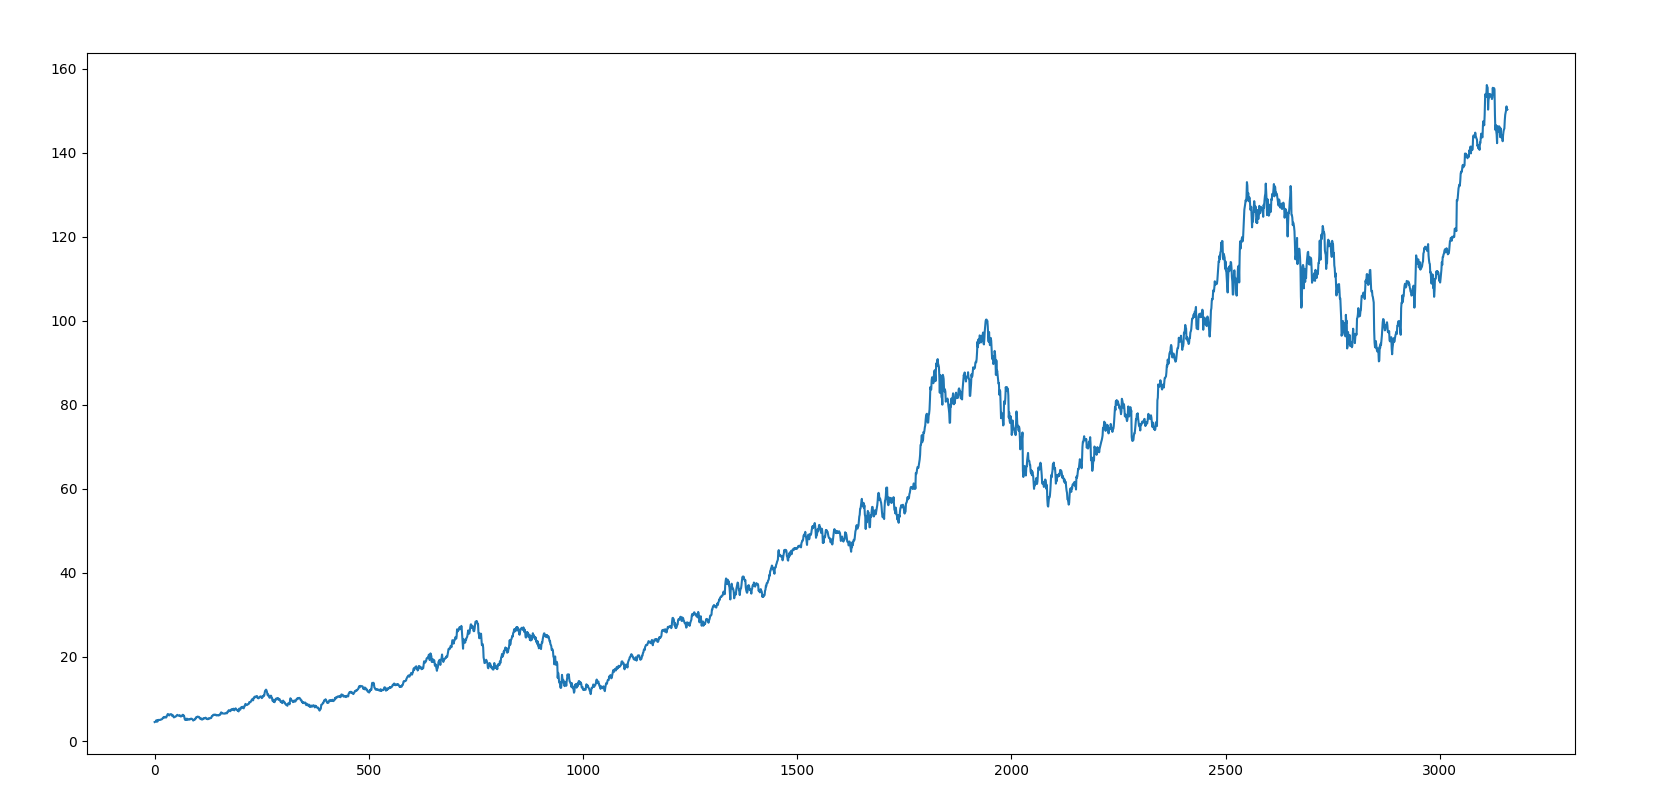
\includegraphics[width=.3\linewidth]{stock1}}
    \subfigure{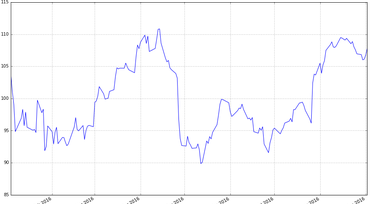
\includegraphics[width=.3\linewidth]{stock2}}
    \subfigure{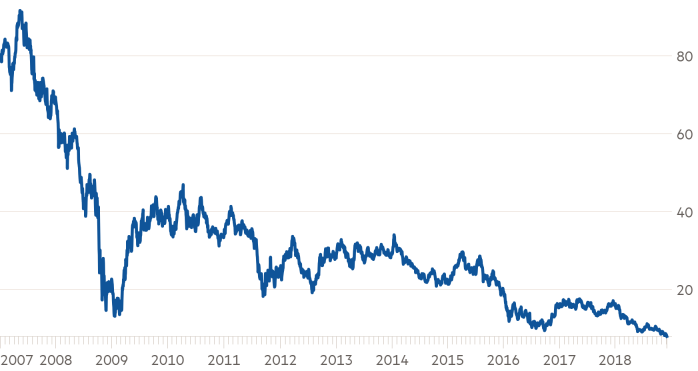
\includegraphics[width=.3\linewidth]{stock3}}
\end{figure}
\end{itemize}
\end{frame}

\begin{frame}{Strategie di investimento}
\begin{itemize}
    \item Generalmente si cerca di comprare quando il titolo ha prezzo basso e vendere quando è alto: \textit{buy} nelle valli e \textit{sell} nei picchi. 
    \item L'operazione va effettuata sul breve periodo (su base giornaliera / settimanale) e ripetuta spesso
    \item È difficile prevedere il preciso andamento e quindi si usano indicatori che lo riassumono
    \item Se si analizza che il mercato è in forte crescita senza eccessive perdite si può optare per BUY-HOLD: compra all'inizio e mantiene il titolo fino alla fine.
    \item Se però il mercato crolla, buy hold segue di conseguenza
\end{itemize}
\end{frame}

\begin{frame}{Strategie di investimento}
\framesubtitle{Strategie più complesse per il breve termine}
\begin{itemize}
    \begin{block}{SMA}
    Simple Moving Average. Strategia che segnala i cambi di tendenza grazie a due medie mobili, una breve (5 / 10 giorni) e una lenta (100 / 200). Le linee delle medie sono tracciate sul grafico dei prezzi e, quando avviene un'intersezione fra le due, si genera un segnale di \textit{buy} o \textit{sell}.\\ Quando la media breve supera quella lenta il segnale è \textit{buy}. Se la media lenta supera quella veloce si ha la situazione opposta e un segnale di \textit{sell}
    \end{block}
    \begin{figure}
        \centering
        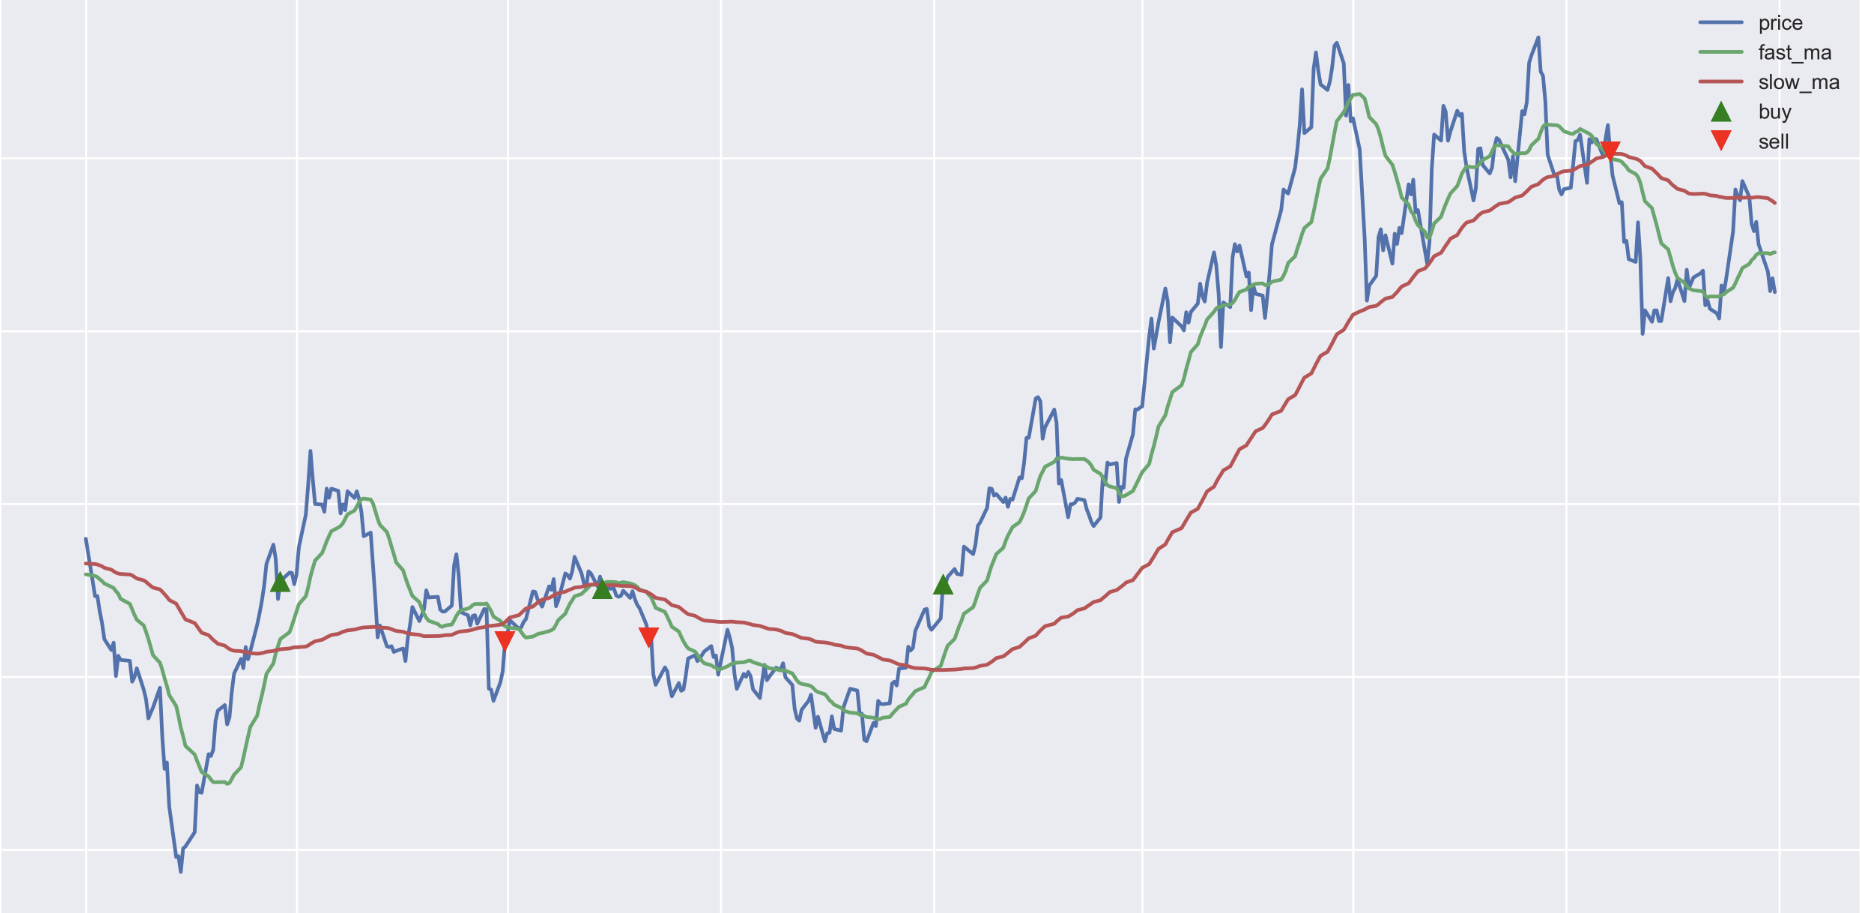
\includegraphics[width=.5\linewidth]{moving_avg2}
    \end{figure}
\end{itemize}
\end{frame}

\begin{frame}{Scopo della tesi}
\begin{itemize}
\item Sentyment AI sceglie in modo intelligente quale strategia applicare a seconda delle varie situazioni,
dell'andamento dei prezzi e del valore degli indcatori.
\item Sentyment AI opera su diverse criptovalute. Ogni criptovaluta ha associato un insieme di AI separate
\item L'obiettivo è sviluppare uno strumento in grado di stabilire, a intervalli di tempo da definire,
quale sia la AI migliore all'interno di ciascun insieme: \textit{meta-learner}
\item Stabilita la migliore, la si può etichettare come "attiva" ed usare in produzione, permettendogli di piazzare direttamente ordini di acquisto e vendita sul mercato.
\end{itemize}
\end{frame}

\begin{frame}{Scelta della migliore AI}
\framesubtitle{\textit{Meta-learner} e \textit{multi-armed bandit}}
\begin{itemize}
\item \textit{Meta-learner} è basato su \textit{multi-armed bandit}, algoritmo di \textit{reinforcement learning}
\item Si allena sulle performance passate di ciascuna AI
\item Parte da inizio dataset e si sposta a step di 250 record. Poi esplora le AI in gioco e calcola per ciascuna \textit{guadagno} e \textit{profitto}
\item A ogni step effettua una scelta: decide se scegliere la AI che finora è stata migliore o se esplorarne una nuova, che potrebbe essere anche meglio
\end{itemize}
\begin{figure}
        \centering
        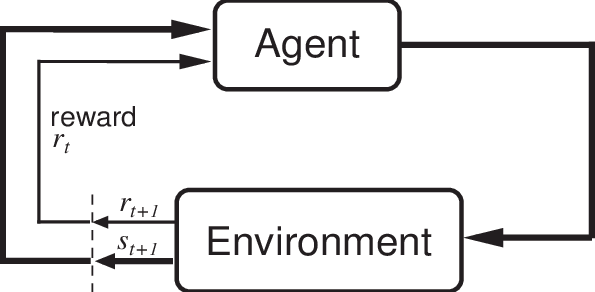
\includegraphics[width=.45\linewidth]{rl}
    \end{figure}
\end{frame}

\begin{frame}{\textit{Meta-learner}}
\begin{itemize}
\item Continuando a registrare le scelte fatte nei vari step, emerge un bandit scelto più spesso di tutti gli altri
\item Dopo un sufficiente numero di step è in grado di dire qual è stata la AI che ha ottenuto performance migliori lungo l'esplorazione
\item Lo stesso algoritmo sarà applicato all'insieme di AI per ciascuna criptovaluta
\item Purtoppo la scarsità di dati non permette iterazioni costanti settimanali o mensili. La scelta è effettuata una sola volta
\end{itemize}
\begin{figure}
        \centering
        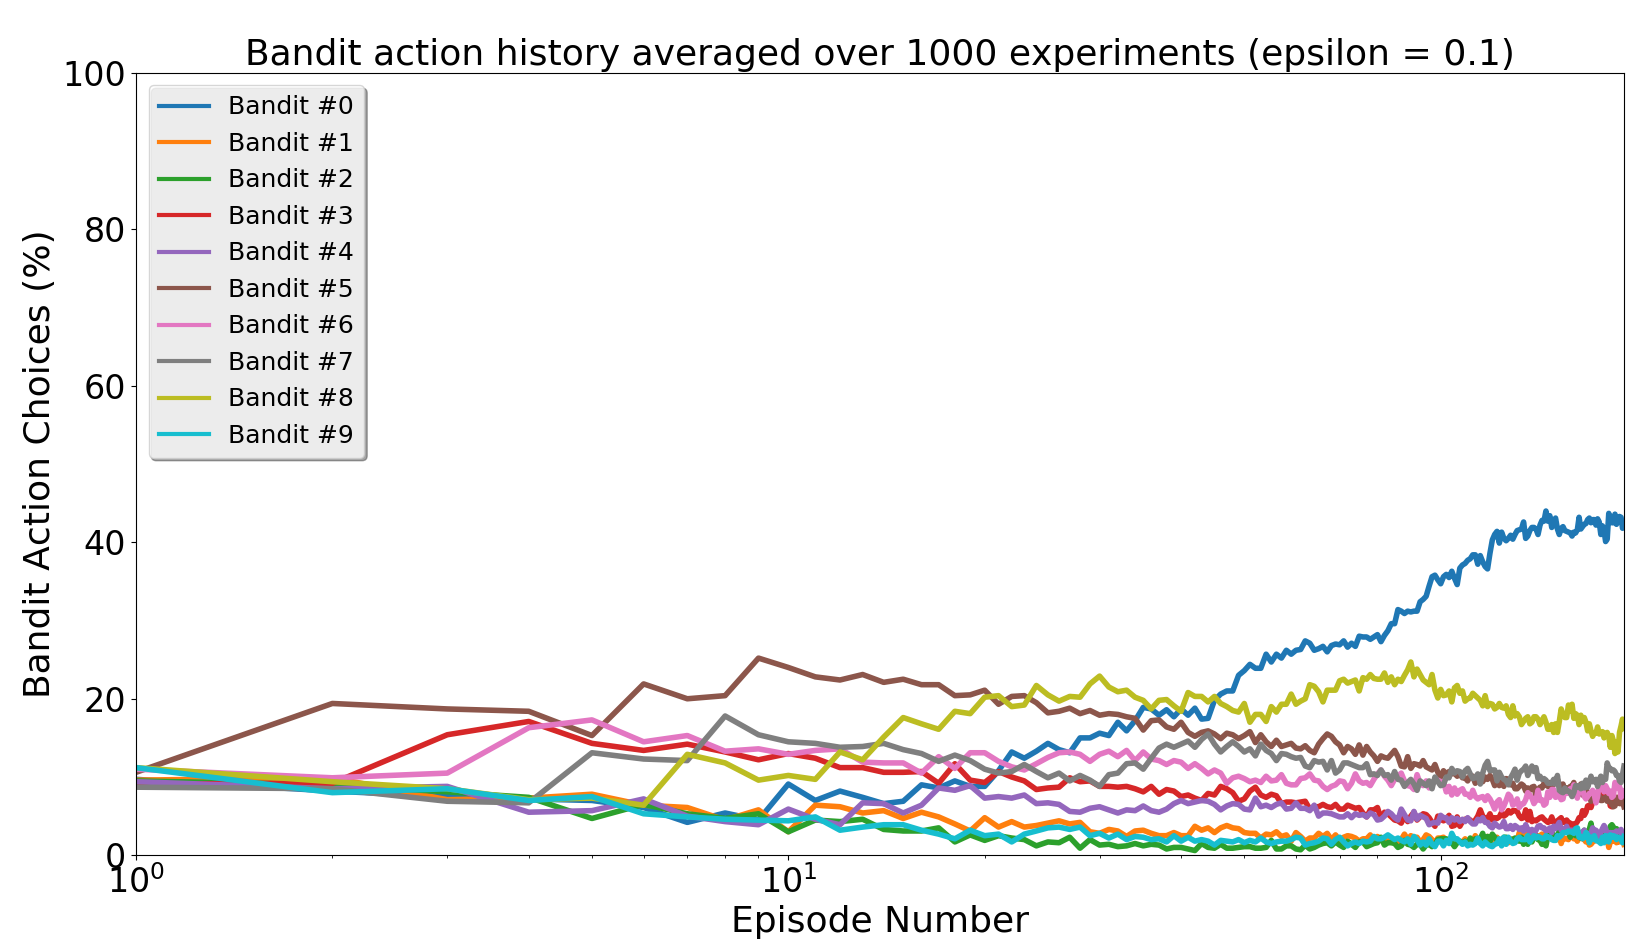
\includegraphics[width=.5\linewidth]{bandit_choice_1000}
\end{figure}
\end{frame}

\begin{frame}{Confronto di Sentyment con altri strumenti}
\begin{itemize}
\item Per confrontare Sentyment si usano strategie di investimento comunemente usate in analisi tecnica
\item Altri strumenti intelligenti di investimento sono proprietari o non esattamente come Sentyment. Comunque difficilmente accessibili
\end{itemize}
\end{frame}

\begin{frame}{Confronto di Sentyment con altri strumenti}
\framesubtitle{\textit{Maximum profit}}
\begin{itemize}
\item asd
\end{itemize}
\end{frame}


\begin{frame}{\textit{Tecnologie e ringraziamenti}}
\end{frame}

\end{document}